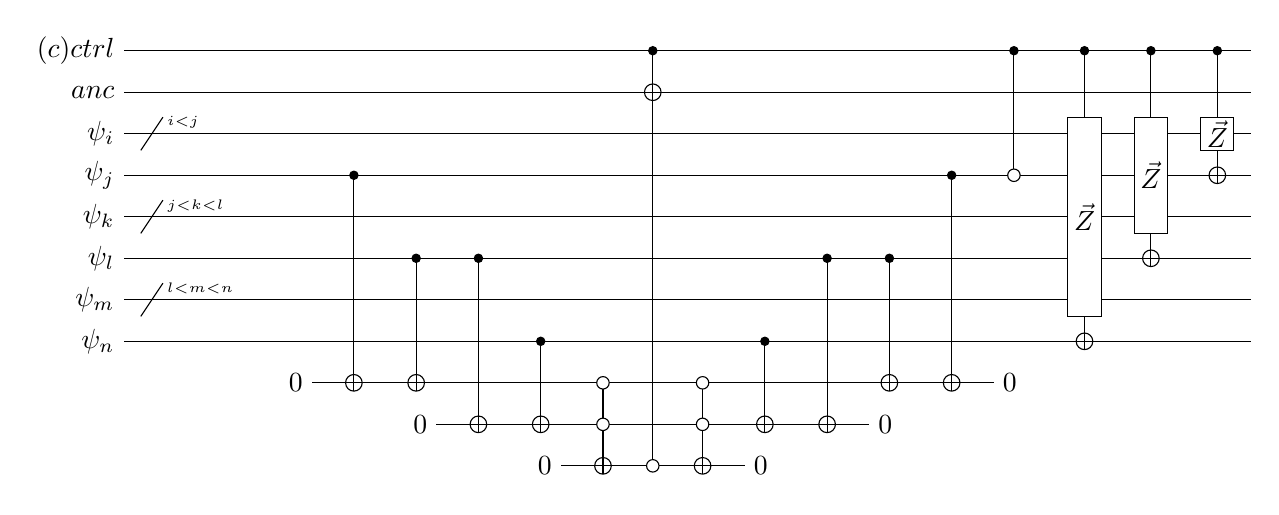
\begin{tikzpicture}[scale=1.000000,x=1pt,y=1pt]
\filldraw[color=white] (0.000000, -7.500000) rectangle (407.000000, 157.500000);
% Drawing wires
% Line 1: ctrl W \text{(c) }ctrl
\draw[color=black] (0.000000,150.000000) -- (407.000000,150.000000);
\draw[color=black] (0.000000,150.000000) node[left] {$\text{(c) }ctrl$};
% Line 2: anc W anc
\draw[color=black] (0.000000,135.000000) -- (407.000000,135.000000);
\draw[color=black] (0.000000,135.000000) node[left] {$anc$};
% Line 3: i W \psi_i
\draw[color=black] (0.000000,120.000000) -- (407.000000,120.000000);
\draw[color=black] (0.000000,120.000000) node[left] {$\psi_i$};
% Line 4: j W \psi_j
\draw[color=black] (0.000000,105.000000) -- (407.000000,105.000000);
\draw[color=black] (0.000000,105.000000) node[left] {$\psi_j$};
% Line 5: k W \psi_k
\draw[color=black] (0.000000,90.000000) -- (407.000000,90.000000);
\draw[color=black] (0.000000,90.000000) node[left] {$\psi_k$};
% Line 6: l W \psi_l
\draw[color=black] (0.000000,75.000000) -- (407.000000,75.000000);
\draw[color=black] (0.000000,75.000000) node[left] {$\psi_l$};
% Line 7: m W \psi_m
\draw[color=black] (0.000000,60.000000) -- (407.000000,60.000000);
\draw[color=black] (0.000000,60.000000) node[left] {$\psi_m$};
% Line 8: n W \psi_n
\draw[color=black] (0.000000,45.000000) -- (407.000000,45.000000);
\draw[color=black] (0.000000,45.000000) node[left] {$\psi_n$};
% Line 9: clean0 W 0 0
\draw[color=black] (60.500000,30.000000) -- (321.500000,30.000000);
% Line 10: clean1 W 0 0
\draw[color=black] (105.500000,15.000000) -- (276.500000,15.000000);
% Line 11: clean2 W 0 0
\draw[color=black] (150.500000,0.000000) -- (231.500000,0.000000);
% Done with wires; drawing gates
% Line 13: i / ^{i<j}
\draw (6.000000, 114.000000) -- (14.000000, 126.000000);
\draw (12.000000, 123.000000) node[right] {$\scriptstyle{^{i<j}}$};
% Line 14: k / ^{j<k<l}
\draw (6.000000, 84.000000) -- (14.000000, 96.000000);
\draw (12.000000, 93.000000) node[right] {$\scriptstyle{^{j<k<l}}$};
% Line 15: m / ^{l<m<n}
\draw (6.000000, 54.000000) -- (14.000000, 66.000000);
\draw (12.000000, 63.000000) node[right] {$\scriptstyle{^{l<m<n}}$};
% Line 16: ctrl anc i j k l m n clean0 LABEL
% Line 17: clean0 START
\draw[color=black] (68.000000,30.000000) node[fill=white,left,minimum height=15.000000pt,minimum width=15.000000pt,inner sep=0pt] {\phantom{$0$}};
\draw[color=black] (68.000000,30.000000) node[left] {$0$};
% Line 18: j +clean0
\draw (83.000000,105.000000) -- (83.000000,30.000000);
\filldraw (83.000000, 105.000000) circle(1.500000pt);
\begin{scope}
\draw[fill=white] (83.000000, 30.000000) circle(3.000000pt);
\clip (83.000000, 30.000000) circle(3.000000pt);
\draw (80.000000, 30.000000) -- (86.000000, 30.000000);
\draw (83.000000, 27.000000) -- (83.000000, 33.000000);
\end{scope}
% Line 19: l +clean0
\draw (105.500000,75.000000) -- (105.500000,30.000000);
\filldraw (105.500000, 75.000000) circle(1.500000pt);
\begin{scope}
\draw[fill=white] (105.500000, 30.000000) circle(3.000000pt);
\clip (105.500000, 30.000000) circle(3.000000pt);
\draw (102.500000, 30.000000) -- (108.500000, 30.000000);
\draw (105.500000, 27.000000) -- (105.500000, 33.000000);
\end{scope}
% Line 20: clean1 START
\draw[color=black] (113.000000,15.000000) node[fill=white,left,minimum height=15.000000pt,minimum width=15.000000pt,inner sep=0pt] {\phantom{$0$}};
\draw[color=black] (113.000000,15.000000) node[left] {$0$};
% Line 21: l +clean1
\draw (128.000000,75.000000) -- (128.000000,15.000000);
\filldraw (128.000000, 75.000000) circle(1.500000pt);
\begin{scope}
\draw[fill=white] (128.000000, 15.000000) circle(3.000000pt);
\clip (128.000000, 15.000000) circle(3.000000pt);
\draw (125.000000, 15.000000) -- (131.000000, 15.000000);
\draw (128.000000, 12.000000) -- (128.000000, 18.000000);
\end{scope}
% Line 22: n +clean1
\draw (150.500000,45.000000) -- (150.500000,15.000000);
\filldraw (150.500000, 45.000000) circle(1.500000pt);
\begin{scope}
\draw[fill=white] (150.500000, 15.000000) circle(3.000000pt);
\clip (150.500000, 15.000000) circle(3.000000pt);
\draw (147.500000, 15.000000) -- (153.500000, 15.000000);
\draw (150.500000, 12.000000) -- (150.500000, 18.000000);
\end{scope}
% Line 23: clean2 START
\draw[color=black] (158.000000,0.000000) node[fill=white,left,minimum height=15.000000pt,minimum width=15.000000pt,inner sep=0pt] {\phantom{$0$}};
\draw[color=black] (158.000000,0.000000) node[left] {$0$};
% Line 24: -clean0 -clean1 +clean2
\draw (173.000000,30.000000) -- (173.000000,0.000000);
\draw[fill=white] (173.000000, 30.000000) circle(2.250000pt);
\draw[fill=white] (173.000000, 15.000000) circle(2.250000pt);
\begin{scope}
\draw[fill=white] (173.000000, 0.000000) circle(3.000000pt);
\clip (173.000000, 0.000000) circle(3.000000pt);
\draw (170.000000, 0.000000) -- (176.000000, 0.000000);
\draw (173.000000, -3.000000) -- (173.000000, 3.000000);
\end{scope}
% Line 25: ctrl -clean2 +anc
\draw (191.000000,150.000000) -- (191.000000,0.000000);
\filldraw (191.000000, 150.000000) circle(1.500000pt);
\draw[fill=white] (191.000000, 0.000000) circle(2.250000pt);
\begin{scope}
\draw[fill=white] (191.000000, 135.000000) circle(3.000000pt);
\clip (191.000000, 135.000000) circle(3.000000pt);
\draw (188.000000, 135.000000) -- (194.000000, 135.000000);
\draw (191.000000, 132.000000) -- (191.000000, 138.000000);
\end{scope}
% Line 26: -clean0 -clean1 +clean2
\draw (209.000000,30.000000) -- (209.000000,0.000000);
\draw[fill=white] (209.000000, 30.000000) circle(2.250000pt);
\draw[fill=white] (209.000000, 15.000000) circle(2.250000pt);
\begin{scope}
\draw[fill=white] (209.000000, 0.000000) circle(3.000000pt);
\clip (209.000000, 0.000000) circle(3.000000pt);
\draw (206.000000, 0.000000) -- (212.000000, 0.000000);
\draw (209.000000, -3.000000) -- (209.000000, 3.000000);
\end{scope}
% Line 27: clean2 END
\draw[color=black] (224.000000,0.000000) node[fill=white,right,minimum height=15.000000pt,minimum width=15.000000pt,inner sep=0pt] {\phantom{$0$}};
\draw[color=black] (224.000000,0.000000) node[right] {$0$};
% Line 28: n +clean1
\draw (231.500000,45.000000) -- (231.500000,15.000000);
\filldraw (231.500000, 45.000000) circle(1.500000pt);
\begin{scope}
\draw[fill=white] (231.500000, 15.000000) circle(3.000000pt);
\clip (231.500000, 15.000000) circle(3.000000pt);
\draw (228.500000, 15.000000) -- (234.500000, 15.000000);
\draw (231.500000, 12.000000) -- (231.500000, 18.000000);
\end{scope}
% Line 29: l +clean1
\draw (254.000000,75.000000) -- (254.000000,15.000000);
\filldraw (254.000000, 75.000000) circle(1.500000pt);
\begin{scope}
\draw[fill=white] (254.000000, 15.000000) circle(3.000000pt);
\clip (254.000000, 15.000000) circle(3.000000pt);
\draw (251.000000, 15.000000) -- (257.000000, 15.000000);
\draw (254.000000, 12.000000) -- (254.000000, 18.000000);
\end{scope}
% Line 30: clean1 END
\draw[color=black] (269.000000,15.000000) node[fill=white,right,minimum height=15.000000pt,minimum width=15.000000pt,inner sep=0pt] {\phantom{$0$}};
\draw[color=black] (269.000000,15.000000) node[right] {$0$};
% Line 31: l +clean0
\draw (276.500000,75.000000) -- (276.500000,30.000000);
\filldraw (276.500000, 75.000000) circle(1.500000pt);
\begin{scope}
\draw[fill=white] (276.500000, 30.000000) circle(3.000000pt);
\clip (276.500000, 30.000000) circle(3.000000pt);
\draw (273.500000, 30.000000) -- (279.500000, 30.000000);
\draw (276.500000, 27.000000) -- (276.500000, 33.000000);
\end{scope}
% Line 32: j +clean0
\draw (299.000000,105.000000) -- (299.000000,30.000000);
\filldraw (299.000000, 105.000000) circle(1.500000pt);
\begin{scope}
\draw[fill=white] (299.000000, 30.000000) circle(3.000000pt);
\clip (299.000000, 30.000000) circle(3.000000pt);
\draw (296.000000, 30.000000) -- (302.000000, 30.000000);
\draw (299.000000, 27.000000) -- (299.000000, 33.000000);
\end{scope}
% Line 33: clean0 END
\draw[color=black] (314.000000,30.000000) node[fill=white,right,minimum height=15.000000pt,minimum width=15.000000pt,inner sep=0pt] {\phantom{$0$}};
\draw[color=black] (314.000000,30.000000) node[right] {$0$};
% Line 35: ctrl -j
\draw (321.500000,150.000000) -- (321.500000,105.000000);
\filldraw (321.500000, 150.000000) circle(1.500000pt);
\draw[fill=white] (321.500000, 105.000000) circle(2.250000pt);
% Line 37: i j k l m G $\vec{Z}$ ctrl +n
\draw (347.000000,150.000000) -- (347.000000,45.000000);
\begin{scope}
\draw[fill=white] (347.000000, 90.000000) +(-45.000000:8.485281pt and 50.911688pt) -- +(45.000000:8.485281pt and 50.911688pt) -- +(135.000000:8.485281pt and 50.911688pt) -- +(225.000000:8.485281pt and 50.911688pt) -- cycle;
\clip (347.000000, 90.000000) +(-45.000000:8.485281pt and 50.911688pt) -- +(45.000000:8.485281pt and 50.911688pt) -- +(135.000000:8.485281pt and 50.911688pt) -- +(225.000000:8.485281pt and 50.911688pt) -- cycle;
\draw (347.000000, 90.000000) node {$\vec{Z}$};
\end{scope}
\filldraw (347.000000, 150.000000) circle(1.500000pt);
\begin{scope}
\draw[fill=white] (347.000000, 45.000000) circle(3.000000pt);
\clip (347.000000, 45.000000) circle(3.000000pt);
\draw (344.000000, 45.000000) -- (350.000000, 45.000000);
\draw (347.000000, 42.000000) -- (347.000000, 48.000000);
\end{scope}
% Line 38: i j k G $\vec{Z}$ ctrl +l
\draw (371.000000,150.000000) -- (371.000000,75.000000);
\begin{scope}
\draw[fill=white] (371.000000, 105.000000) +(-45.000000:8.485281pt and 29.698485pt) -- +(45.000000:8.485281pt and 29.698485pt) -- +(135.000000:8.485281pt and 29.698485pt) -- +(225.000000:8.485281pt and 29.698485pt) -- cycle;
\clip (371.000000, 105.000000) +(-45.000000:8.485281pt and 29.698485pt) -- +(45.000000:8.485281pt and 29.698485pt) -- +(135.000000:8.485281pt and 29.698485pt) -- +(225.000000:8.485281pt and 29.698485pt) -- cycle;
\draw (371.000000, 105.000000) node {$\vec{Z}$};
\end{scope}
\filldraw (371.000000, 150.000000) circle(1.500000pt);
\begin{scope}
\draw[fill=white] (371.000000, 75.000000) circle(3.000000pt);
\clip (371.000000, 75.000000) circle(3.000000pt);
\draw (368.000000, 75.000000) -- (374.000000, 75.000000);
\draw (371.000000, 72.000000) -- (371.000000, 78.000000);
\end{scope}
% Line 39: i G $\vec{Z}$ ctrl +j
\draw (395.000000,150.000000) -- (395.000000,105.000000);
\begin{scope}
\draw[fill=white] (395.000000, 120.000000) +(-45.000000:8.485281pt and 8.485281pt) -- +(45.000000:8.485281pt and 8.485281pt) -- +(135.000000:8.485281pt and 8.485281pt) -- +(225.000000:8.485281pt and 8.485281pt) -- cycle;
\clip (395.000000, 120.000000) +(-45.000000:8.485281pt and 8.485281pt) -- +(45.000000:8.485281pt and 8.485281pt) -- +(135.000000:8.485281pt and 8.485281pt) -- +(225.000000:8.485281pt and 8.485281pt) -- cycle;
\draw (395.000000, 120.000000) node {$\vec{Z}$};
\end{scope}
\filldraw (395.000000, 150.000000) circle(1.500000pt);
\begin{scope}
\draw[fill=white] (395.000000, 105.000000) circle(3.000000pt);
\clip (395.000000, 105.000000) circle(3.000000pt);
\draw (392.000000, 105.000000) -- (398.000000, 105.000000);
\draw (395.000000, 102.000000) -- (395.000000, 108.000000);
\end{scope}
% Done with gates; drawing ending labels
% Done with ending labels; drawing cut lines and comments
% Done with comments
\end{tikzpicture}
